\chapter{Implementation}
\label{c:implementation}

In this section, the implementation that was used for the experiment is discussed.
In section \ref{s:tag} the implementation of the tags is presented.
Section \ref{s:app} is about the implementation of the App.

\section{Tag}
\label{s:tag}
The software of the tags consits of n modules:
\begin{enumerate}
	\item Temperature and humidity sensor
	\item Gyroscope
	\item Two way ranging
	\item UWB network
	\item BLE communication
	\item Job handler
\end{enumerate}
The following subsections will discuss the first five modules, followed by how they interact using the job handler module.
The section \ref{ss:combination} discusses chalanges from combining these modules and how they were solved.

\subsection{Temperature and humidity module}
\label{ss:temp_hum_module}
This module is responsible for managing the DHT22 humidity and temperature sensor.
It is responsible to setup the sensor during initial startup and to provide the sensors measurements when queried.
The DHT22 sensor communicates using only one data pin, pin 13, which will be referd to as the data pin in this section.
Dmitry Sysoletin created an implementation \ref{sysoletin2021nrf52_dht11} for the DHT11 sensor together with the nRF52840 board that build the basis for this implementation, by addapting it to the DHT22 and adding functionalities needed by the job handler module.


Since the DHT22 is a very simple sensor, using single bus comunication, not much setup is needed.
The evaluation of the sensor data requires that the voltage of the pin is read out in pre-defined intervals, when reading the sensor data.
To do this, a clock is required.
This resource has to be reserved an initiated at startup.
This is the only setup that is required for the DHT22 sensor.


To initiate a sensor-read the voltage of the data pin is set to 0.
When the sensor is in standby mode, the data pin is on \textit{logic high}, and when set to \textit{logic low}, the sensor will respond with a read of its current value.
A schematc view of a sensor read of the DHT22 can be seen in Figure \ref{f:dht22_signal}.
The temperature and humidity module will then check the Pin State in intervals of 5ms, until a \textit{logic low} is registered, signalling that the sensor has registered the request. 
The module will now monitor the pin state, waiting for \textit{logic low} followed by a \textit{logic high}, this beeing the start condition of the data transfer. \\
The data is transfered in five chunks of eight bits.
Each bit is preceeded by a prolonged \textit{logic low} state, that is detected by the module
The module then proceeds to write the state of the data pin into a 8-bit buffer, \textit{logic high} corresponding to a 1 and \textit{logic low} to 0.\\
Once all five chunks are read, the communication has ended and the module can verify the data.
The first two bytes correspond are combined to form the temperature information in celcius, the second and third form the humidity.
Both values are multiplied by 100 and stored in a 16-bit integer. This doesn't loose data, since the sensor only measures up to a precision of 1 after the decimal point.
The data beeing stored in an integer help with data transfer.
It will be converted back on the phone.
The fith chunk contains the parity and is used to accept or reject the humidity and temperature values.
If the process fails at any state, -100\degree C is returned for the temperature and -100% for humidity.
These form both impossible values, since humidity can't be negative and the DHT22 sensor can only detect temperatures as low as -20\degree C.


\begin{figure}[ht!]
\centering
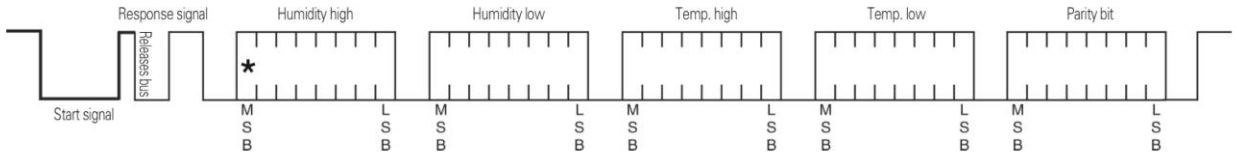
\includegraphics[width=\linewidth]{graphics/DHT22_signal.png}
\caption{Signal of a DHT22 sensor-read as presented in the manual \cite{AM2302}.}
\label{f:dht22_signal}
\end{figure}

\subsection{Gyroscope}
\label{ss:gyro_module}
This module manages the MPU6050 gyroscope and accelerometer.
It is responsible to setup the sensor and report its result.
An implementation for the MPU6050 was present in the nRF52 15.3.0 SDK, but is no longer avaliable for the nRF52 17.1.0 SDK, used in this project.
The old implementation was ported to this project.
This consisted of replacing deprecated parts of the SDK with updated ones and adding newly required flags to the build.


MPU6050 sensors use the I2C communication protocol.
The nRF52 SDK does not include an implementation for this protocol, but has a Two Wire Interface (TWI) implementation that is compatible with the I2C protocol.
During startup the TWI module has to be initialized.
This is handled by the SDK, but requires some parameters to be passed.
\begin{itemize}
	\item The Serial Clock Line (SCL) defines what pin will be used for the clock shared in the TWI. This implementation uses pin 11.
	\item The Serial Data Line (SDA) defines which pin is used for the data communication. Pin 12 was used.
	\item The frequency which the TWI uses. It is defined in MPU6050 data sheet, and is 100 kHz \cite{MPU6050}.
	\item The Interrupt priority is a rank that determins, how easyely this process can cause an interrupt. It is set to high.
\end{itemize}
After the TWI service is initiated with these parameters, it is enabled, ensuring that its resources are locked and can not be used by other services.


Afterwards the results from the sensor can be read using the TWI service again.
The TWI-TX requires the adress of the read device and a registry where to write the MPU6050 datasheet \cite{MPU6050}.
The adress of the sensor is the same for all MPU6050 sensors and can be found in the manua
It sets a flag to true once the sensor has writen the data, which then can be read using the TWO-RX function.
The result consist of three 16-bit integers, representing the angular velocity arround the X,Y and Z axis, shown in figure \ref{f:MPU6050_orientation}.\\
Returning this data when queried has only limited use.
It represents a measurement of the current situation.
The caller is more interested what happened since the last query.
Two different implementations for the read of the gyroscope were used during the experimental phase of this thesis.
One would try to return the current orientation of the tag. This read will be called the orientational read.
 while the other would return the maximal registered angular velocity since the last read.




\begin{figure}[ht!]
\centering
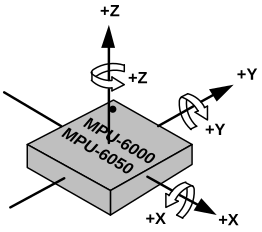
\includegraphics[width=200px]{graphics/MPU6050_orientation.png}
\caption{Schematic view of the MPU6050, showing the direction of the three axis X,Y,Z.}
\label{f:MPU6050_orientation}
\end{figure}


\section{Combining modules}
\label{ss:combination}


\section{App}
\label{s:app}
Nordic Semi Conductors, the maker of the used microcontrolers, published the code to a simple app that allows for BLE communication with their devices.
It is called nRF Toolbox.
It is intended to pair with the ble\_ app\_ uart example, published in the nRF52 SDK.
Since this example code was used as the basis for the ble communication used in this project, it was addapted to work with this project.


The App contains different modules, intended for different examples, among them the Universal Asynchronus Receiver/Transmitter (UART) module (see \ref{f:Toolbox_modules}).
It is intended to be used with the ble\_ app\_ uart example.
When opem it shows the ble services that are currently beeing addvertised and allows the user to connect to one of them \ref{f:Toolbox_connect}.
It then opens a window similar to phone messangers, were the keyboard can be used to tpye messages, that are sent to the connected devices.

\begin{figure}[ht!]
\centering
 \caption{nRF Toolbox module menue, with the added Art Tracking Module}
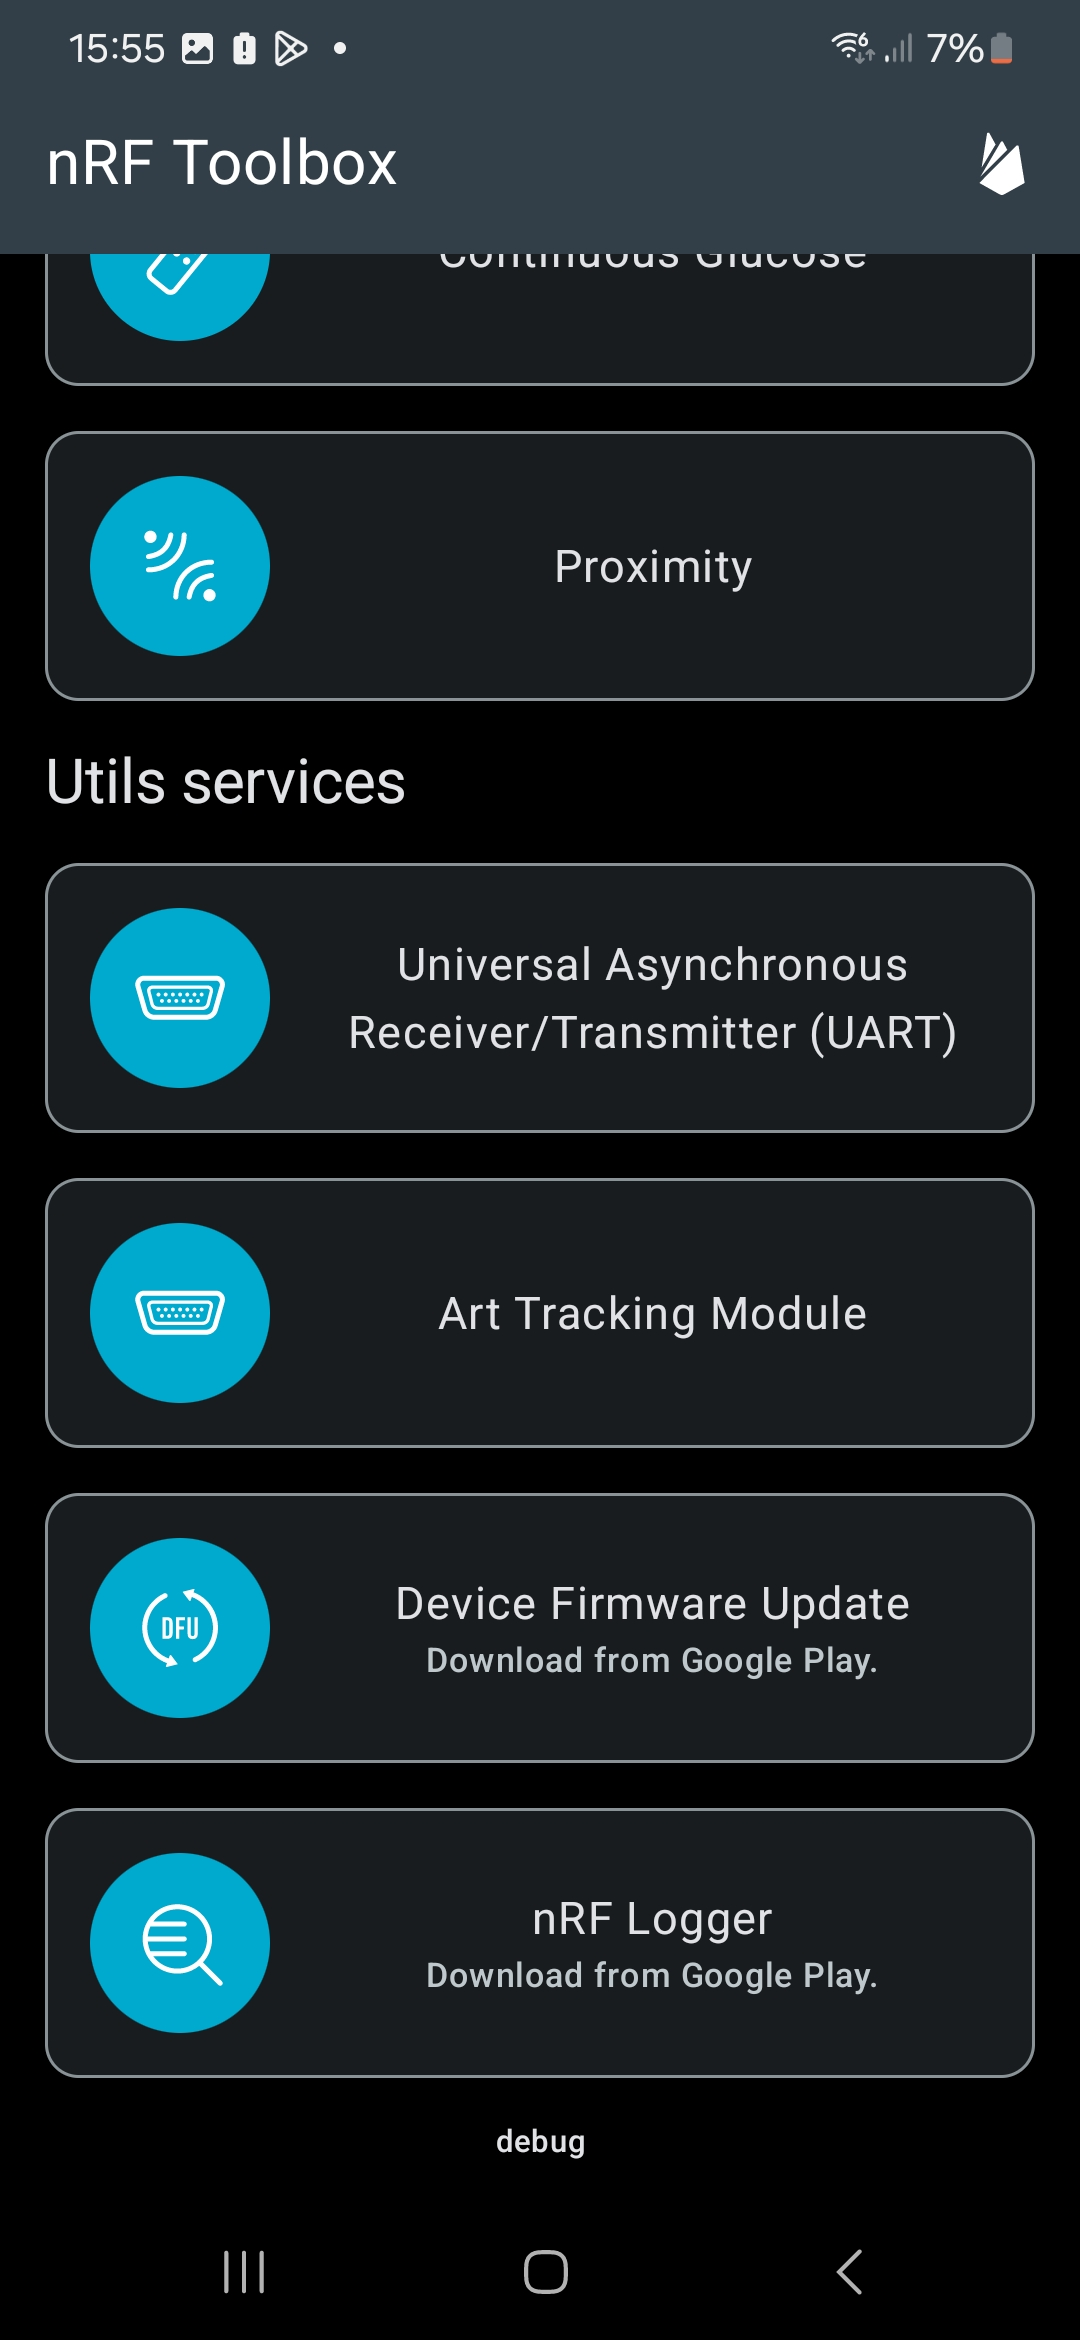
\includegraphics[width=200px]{graphics/nRF_toolbox_modules.jpg}
\label{f:Toolbox_modules}
\end{figure}

\begin{figure}[ht!]
\centering
 \caption{nRF Toolbox shows avaliable devices to connect to}
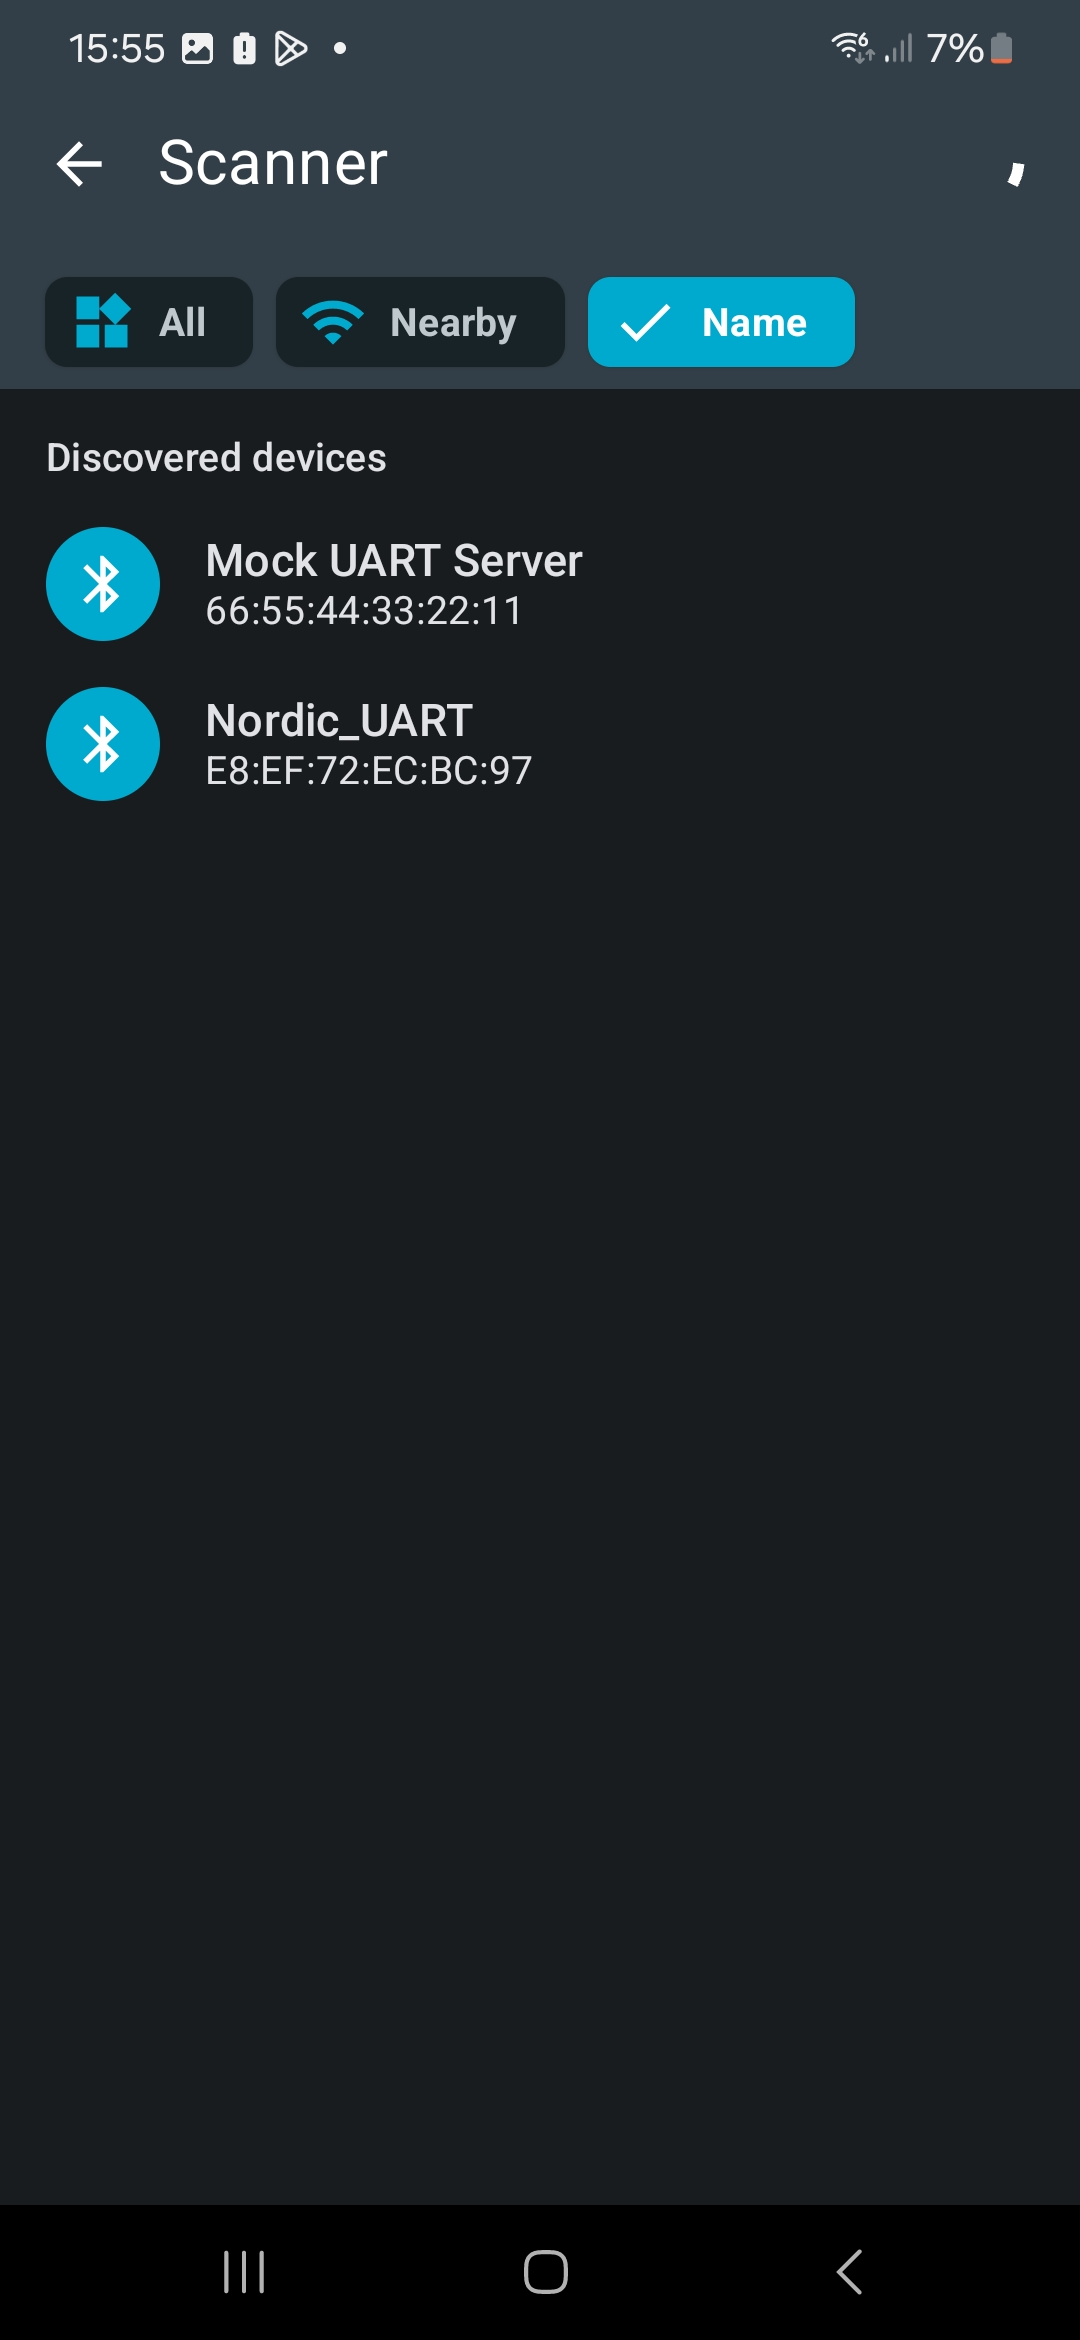
\includegraphics[width=200px]{graphics/nRF_toolbox_connect.jpg}
\label{f:Toolbox_connect}
\end{figure}

\begin{figure}[ht!]
\centering
 \caption{nRF Toolbox UART module screen}
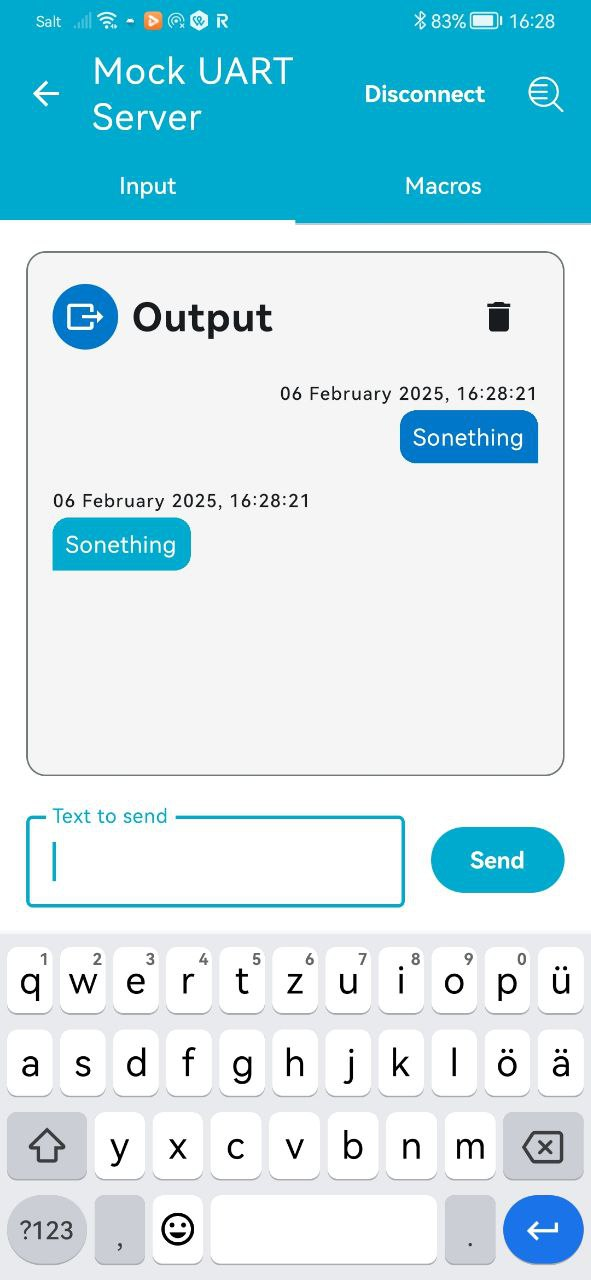
\includegraphics[width=200px]{graphics/nRF_toolbox_messanger.jpg}
\label{f:Toolbox_connect}
\end{figure}

Since the development of an application was not the primary focus of this thesis, it was decided to take the nRF Toolbox app and add a new module for art-traking to it.
The UART module searved as the basis for this new module, since it had a lot of usefull services already implemented.
As with the UART module the art-tracking module opens up the same connection page \ref{f:Toolbox_connect}, that allows the user to select the art-tracking and connect to it.

Once connected, the observation screen is shown (figure \ref{f:Toolbox_art_tracking_empty}).
At the bottom seven parameters can be set: \textit{time}, \textit{max Temp}, \textit{min Temp}, \textit{max Hum}, \textit{min Hum}, \textit{max Angle}, \textit{max Dist}.
The parameters \textit{max}/\textit{min} \textit{Temp}/\textit{Hum} represent the expected range of humidity and temperature.
Any measurement outside these parameter will be considered a dangerous value by the app.
The tollerated difference in angle compared to the previous measurement is set by \textit{max Angle}, larger differences are considered dangerous values.
Distance measurement work analogously with \textit{max Dist} in meters.
The \textit{time} set defines the time that passes enbetween measurements in seconds.
The default is set to 350 seconds.
This means that the time that passes between, for example, the temperature measurements on tag 2 are 350 seconds.


\begin{figure}[ht!]
\centering
 \caption{Art Tracking module oberservation screen before measurements}
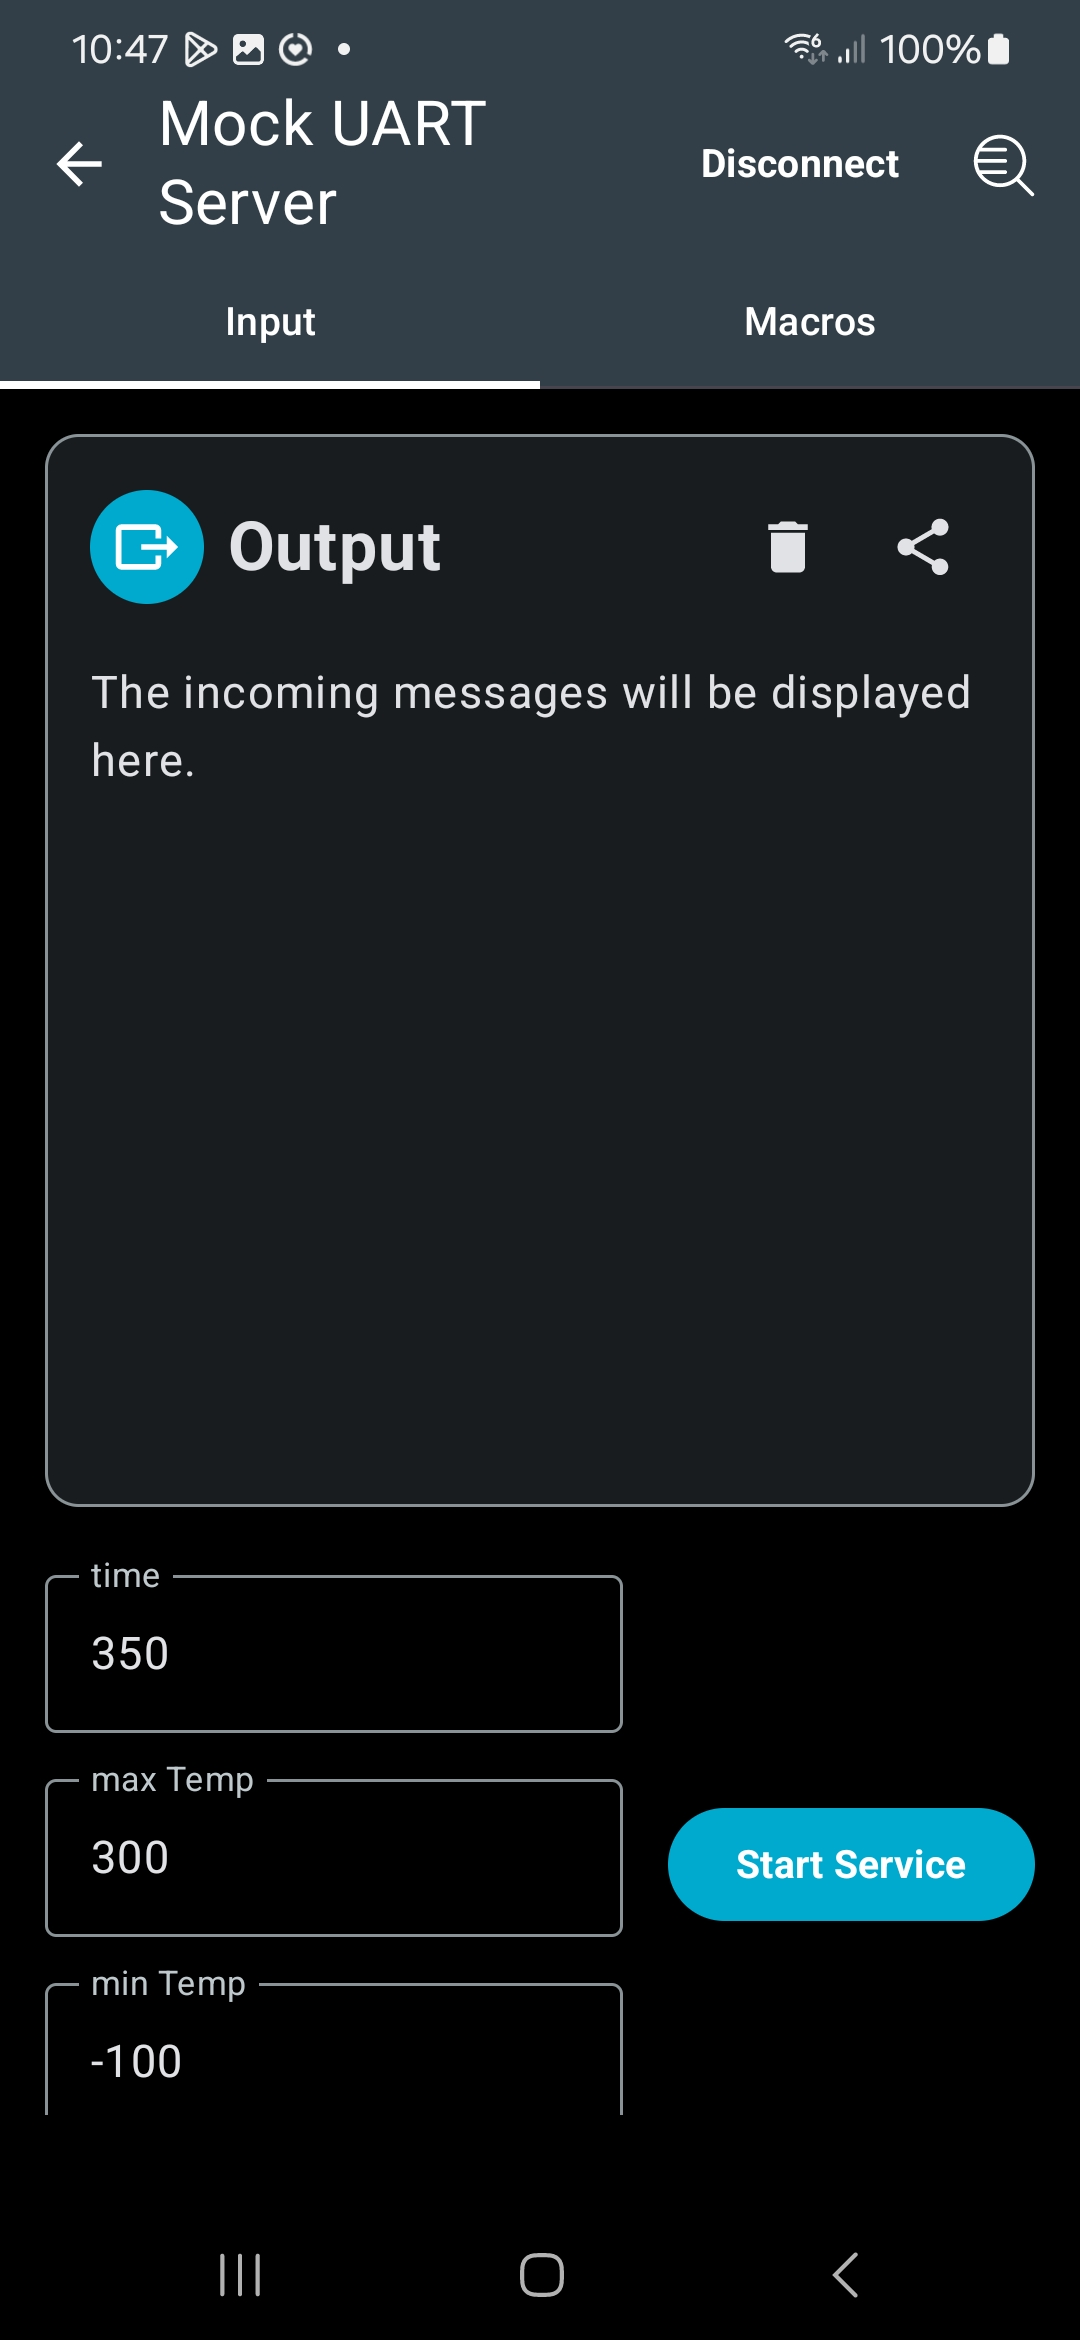
\includegraphics[width=200px]{graphics/nRF_toolbox_art_tracking_empty.jpg}
\label{f:Toolbox_art_tracking_empty}
\end{figure}


When the user presses the \textit{Start Service} button, a services starts that poeriodically queries the tags for the Measurements.
Figure \ref{code:App_main_loop} shows the measurement loop.
Each sensor is assigned a character.
\textit{T} for temperature and humidity, \textit{G} for gyro and \textit{D} for distance.
Each tag has a number, here from one to four since four tags were used in the experiments.
The loop concatenates these two characters and sends the resulting query to the connected tag.
Then the next tag-number is prepared for the next query.
Once all tags have been queried for a sensor, the tag-number starts with the first again and the next sensor is queried.
In between cals the app waits.
The call time for distance-measurement is fixed at 80 seconds.
Distance measurement takes longer than the other sensors, since for every devices three measurements need tobe conducted.
Additionaly the sensors that do not participate in a ranging session are sleeping for a quite generous amount of time, to ensure they don't distrub the ranging session.
80 seconds has been chosen, since it allows enough time for all the ranging to happen, plus two repeats per sensor in case the ranging session fails.
For the other sensors the waiting time in between queries is calculated from the remaining set time, after the ranging time is deducted.

\begin{figure}[h]
    \centering
    \begin{lstlisting}[language=Java]
    private val sensors = listOf("T", "G", "D")
    private val devices = listOf("1", "2", "3", "4")
    private var measurement_type = 0
    private var tag = 0
    private var timeBetweenCals: Long = 3750

    private val runnable = object : Runnable {
        override fun run() {
            if (tag >= list2.size) {
                tag = 0
                measurement_type += 1
            }
            if (measurement_type >= list1.size) {
                measurement_type = 0
            }
            val textToSend = "${list1[measurement_type]}${list2[tag]}"
            artRepository.sendText(textToSend, MacroEol.LF)
            tag += 1
            if(list1[measurement_type] == "D"){
                handler.postDelayed(this, 80000)
            } else {
                handler.postDelayed(this, timeBetweenCals)
            }
        }
    }
    \end{lstlisting}
    % Optionally, add a caption to the figure
    \caption{Section from the ArtMetricService.kt, main measurement loop}
	\label{code:App_main_loop}
\end{figure}

Once the process has started, the queries will appear in the chat window on the right side of the screen.
The responses are on the right side, see figure \ref{code:App_main_loop}.
If the response is inside the set parameters, the message bubble will appear blue.
If the measured value is considered a dangerous value, the text bubble will appear red (see figure \ref{f:Toolbox_art_filled}).
Since the message display is programmed in a asynchronus way, it can happen, that the answer to a query appears before the querry itself, if the querried tag is the same as the connected tag.
The service can be stopped by pressing the \textit{start service} button again or by exiting this screen in any way.


\begin{figure}[ht!]
\centering
 \caption{Art Tracking module, queries and responses}
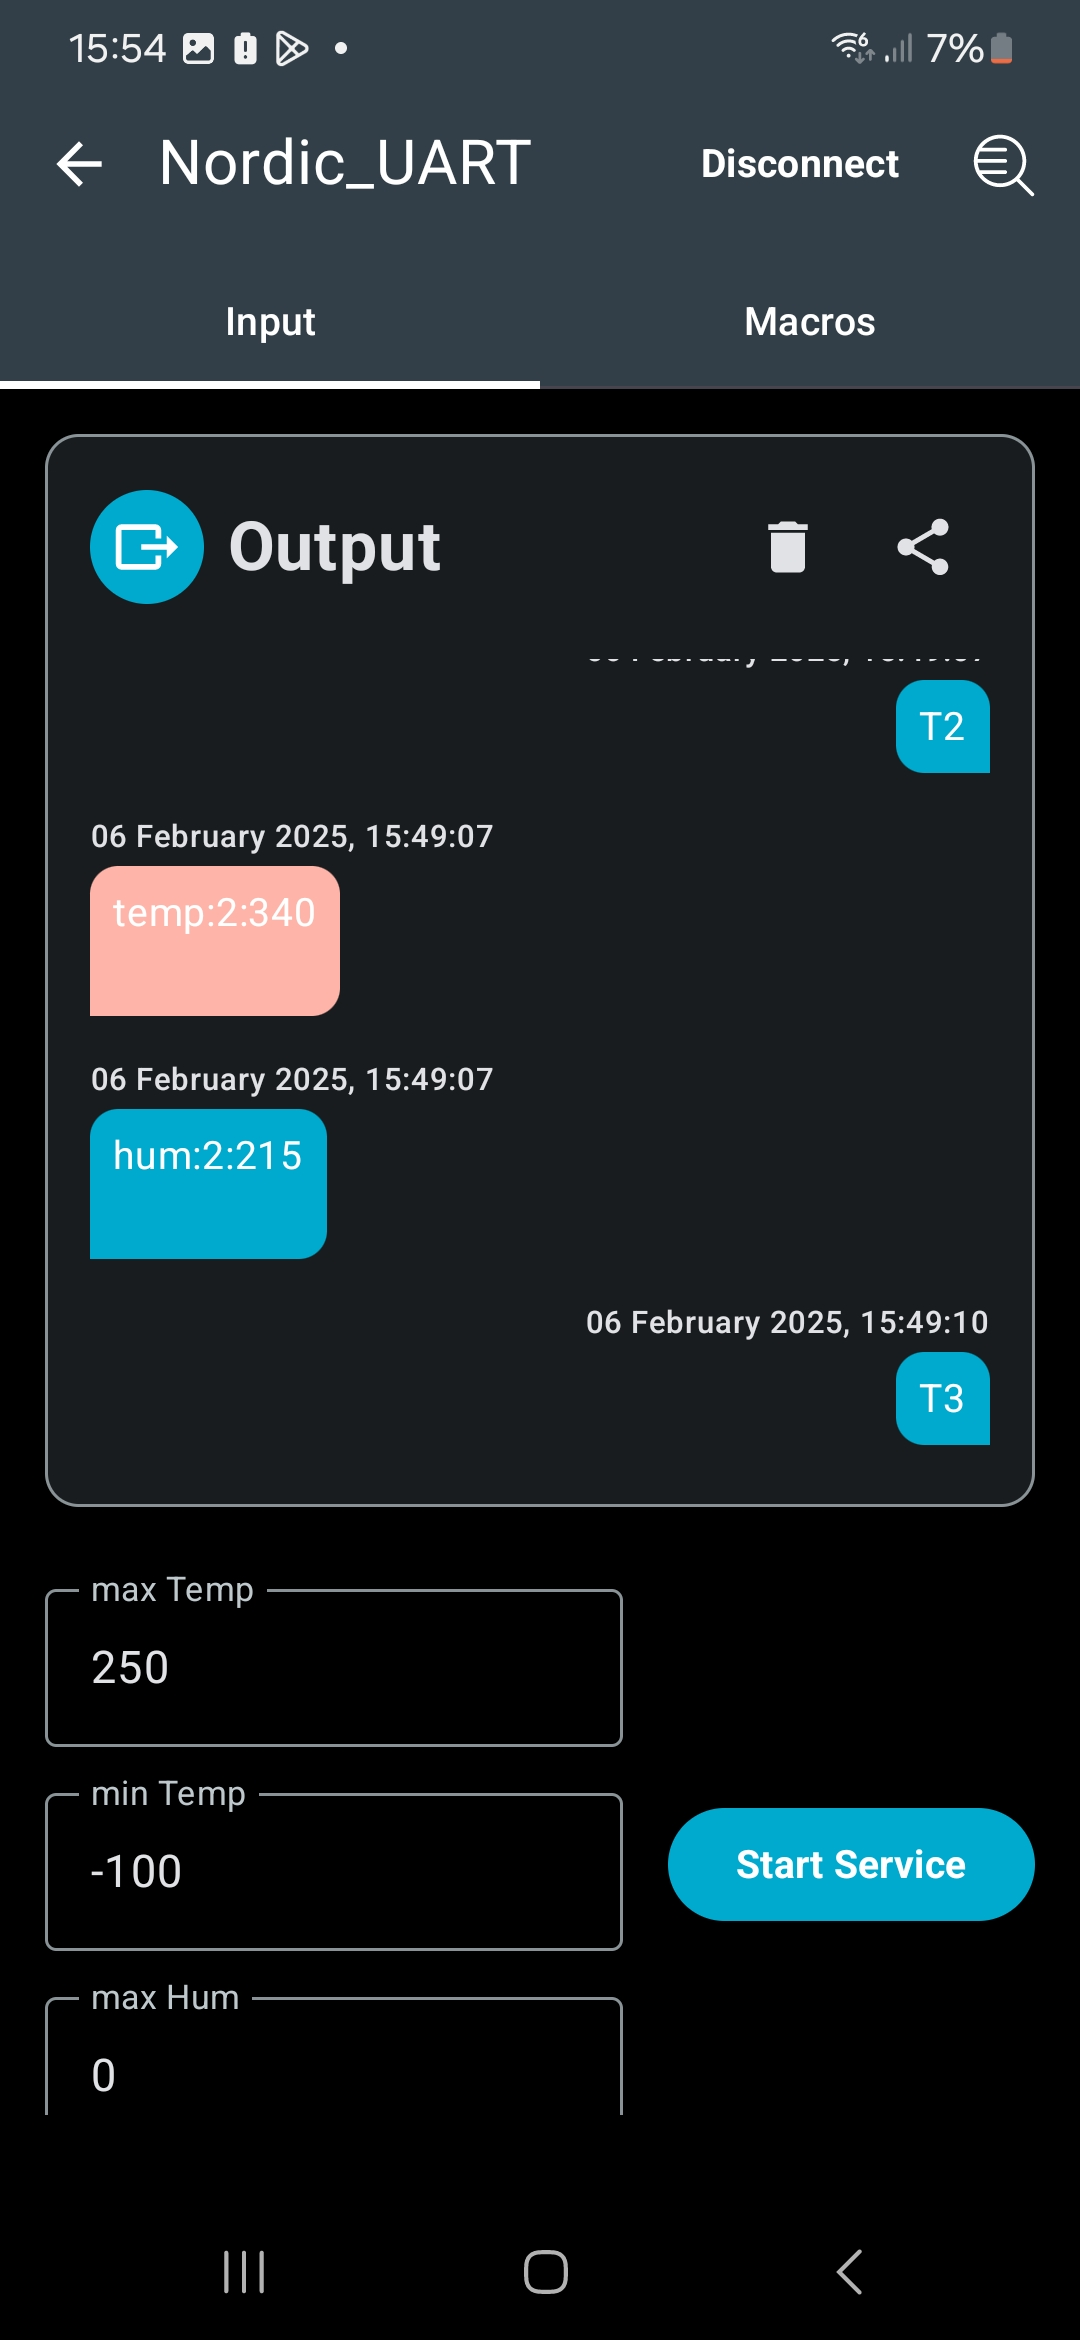
\includegraphics[width=200px]{graphics/nRF_toolbox_Bad_Value_2.jpg}
\label{f:Toolbox_art_filled}
\end{figure}


%TODO: add image that shows an example file
The query-answers are appended to a file that is safed in the app-storage.
The information appendded consits of: the queried tag, the returned values, a timestamp and if the value was unproblematic.
This functionality is intended for experimental evaluation. 
In a real word application, this data should be periodically backed up on a server in a compressed manner.
When pressing the share-button on the top right of the message-box \ref{f:Toolbox_art_filled}.
It will open the Android naitive share functionality, to share the file over mail, an installed messanger, save it to onedrive or send it over Bluetooth.
In this project all files were sent with email.
Pressing the trashcan next to it will delete the chat and empty the file.
This allows the user to distinguish between different testing session.